\documentclass{report}

\usepackage[utf8]{inputenc}
\usepackage[english, russian]{babel}
\usepackage{geometry}
\usepackage{listings}
\usepackage[T2A]{fontenc}
\usepackage[14pt]{extsizes}
\usepackage{color}
\usepackage{graphicx}
\usepackage[titles]{tocloft}
\usepackage[hyphens]{url}
\usepackage{indentfirst}

\geometry{a4paper,top=2cm,bottom=2cm,left=2cm,right=1.5cm}
\setlength{\parskip}{0.5cm}
\setcounter{tocdepth}{4}
\setcounter{secnumdepth}{4}
\sloppy

\definecolor{darkgreen}{rgb}{0.0, 0.5, 0.0}
\lstset{
    language=C++,
    basicstyle=\footnotesize,
    numbers=left,
    numberstyle=\tiny,
    numberfirstline=true,
    numbersep=5pt,
    keywordstyle=\color{blue}\bfseries,
    commentstyle=\color{darkgreen},
    stringstyle=\color{red},
    showspaces=false,
    showstringspaces=false,
    captionpos=t,
    breaklines=true,
    breakatwhitespace=false,
    extendedchars=true,
    frame=tb,
    title=\lstname,
}

\begin{document}
    \begin{titlepage}

        \begin{center}
            \textbf{Федеральное государственное автономное образовательное учреждение высшего образования} \\
            "Национальный исследовательский Нижегородский государственный университет им. Н.И. Лобачевского" (ННГУ) \\
            \textbf{Институт информационных технологий, математики и механики}

            \vspace{\fill}

            \textbf{\LargeОтчет по лабораторной работе \\}
            \textbf{\large\\ «Поразрядная сортировка для вещественных чисел (тип double) с четно-нечетным слиянием Бэтчера»}

            \vspace{\fill}

            \hfill\parbox{8cm}{
                \hspace*{5cm}\hspace*{-5cm}\textbf{Выполнил:} \\ Студент группы 381708-1 \\ Коннов Сергей Юрьевич \\ \\ \\
                \hspace*{5cm}\hspace*{-5cm}\textbf{Проверил:}\\ Доцент кафедры МОСТ, \\ кандидат технических наук \\ Сысоев А. В.
                \hbadness=20000
            }

            \vspace{\fill}

            Нижний Новгород \\ 2020 г.
        \end{center}

    \end{titlepage}

    % =============================================
    % Оглавление
    % =============================================
    \setcounter{page}{2}
    \setlength{\cftsecindent}{0em}
    \setlength{\cftsubsecindent}{1.25em}
    \setlength{\cftsubsubsecindent}{2.5em}
    \setlength{\cftsubsubsecnumwidth}{1.25em}
    \tableofcontents

    \newpage
    % =============================================
    % Введение
    % =============================================
    \section*{Введение}
    \addcontentsline{toc}{section}{Введение}
    \par Поразрядная сортировка - алгоритм  сортировки, который выполняется за линейное время. Алгоритм применим для сортировки любых объектов, запись которых можно поделить на "разряды", содержащие сравнимые значения, например целые и вещественные числа, строки, являющиеся набором символов, и вообще произвольные значения в памяти, представленные в виде набора байт.
    \par Для эффективного распараллеливания можно разделить входной массив на несколько частей, для каждой части параллельно выполнить поразрядную сортировку, а затем слить их в единый отсортированный массив, например, с помощью чётно-нечётного слияния Бэтчера.
    \par В данной работе необходимо изучить алгоритм поразрядной сортировки вещественных чисел с чётно-нечётным слияния Бэтчера и реализовать последовательные и параллельные версии алгоритма с использованием различных технологий выполнения параллельных вычислений.

    \newpage
    % =============================================
    % Постановка задачи
    % =============================================
    \section*{1. Постановка задачи}
    \addcontentsline{toc}{section}{1. Постановка задачи}
    В ходе данной лабораторной работе требуется:
    \begin{itemize}
        \item изучить алгоритмы поразрядной сортировки вещественных чисел и чётно-нечётного слияния Бэтчера;
        \item реализовать последовательную версию алгоритма;
        \item реализовать параллельные с использованием:
        \begin{itemize}
            \item OpenMP
            \item TBB
            \item \verb|std::thread|
        \end{itemize}
        \item провести вычислительные эксперименты и сделать выводы об эффективности разработанных реализаций.
    \end{itemize}

    \newpage
    % =============================================
    % Описание алгоритма
    % =============================================
    \section*{2. Описание алгоритма}
    \addcontentsline{toc}{section}{2. Описание алгоритма}

    \par Существует две различных модификации данного алгоритма - Least Significant Digit (LSD) и Most Significant Digit (MSD). При сортировке LSD порядок сортировки идёт от младших разрядов к старшим. При MSD порядок обратный - от старших разрядов к младшим. В данной работе рассматривается только алгоритм LSD.
    \par В ходе поразрядной сортировки каждое число делится на некоторое число разрядов. Каждый разряд включает в себя несколько битов. Для каждого разряда вызывается последовательно сортировка подсчётом. Для вещественных чисел можно использовать разделение по байтам.
    \par Вещественные числа двойной точности (double) в памяти представляются следующим образом: старший бит отвечает за знак (0 - положительное число и 1 - отрицательное), следующие 11 бит представляют порядок числа, оставшиеся 52 бита отвечают за представление мантиссы.
    \par В ходе поразрядной сортировки для каждого байта чисел входного массива последовательно, начиная с младшего байта, применяется сортировка подсчётом. Для первых 7 байтов различий между отрицательными и положительными числами не делается.
    Числа в массиве перезаписываются по возрастанию значения очередного байта. Последний байт кодирует также знак числа, поэтому для него работа сортировки подсчётом изменена: байты со значением 0-127 (положительные) записываются по возрастанию, а байты со значением 128-255 (отрицательные) -- по убыванию.

    \newpage
    % =============================================
    % Описание схемы распараллеливания
    % =============================================
    \section*{3. Описание схемы распараллеливания}
    \addcontentsline{toc}{section}{3. Описание схемы распараллеливания}
    \par Исходный массив равномерно разбивается на количество частей, равное числу потоков. Каждый поток производит поразрядную сортировку для своей части массива. После выполнения сортировки части массива сливаются с использованием алгоритма чётно-нечетного слияния Бэтчера.
    \par Алгоритм Бэтчера заключается в следующем: два упорядоченных массива, которые необходимо слить, разделяются на элементы с чётными и нечётными индексами. Такое слияние может быть выполнено параллельно. Чтобы массив стал окончательно отсортированным, достаточно сравнить пары элементов, стоящие на нечётной и чётной позициях.
    \newpage
    % =============================================
    % Описание программной реализации
    % =============================================
    \section*{4. Описание программной реализации}
    \addcontentsline{toc}{section}{4. Описание программной реализации}
    \par В ходе программной реализации было принято решение использовать распараллеливание на уровне задач. Во всех параллельных реализациях были созданы задачи следующих типов:
    \begin{itemize}
        \item Сортировка элементов массива с индексом первого элемента \verb|l| и размером \verb|size|;
        \item Слияние чётных элементов двух частей массива с индексами первых элементов \verb|l1|, \verb|l2| и размерами \verb|size1|, \verb|size2|;
        \item Слияние нечётных элементов двух частей массива с индексами первых элементов \verb|l1|, \verb|l2| и размерами \verb|size1|, \verb|size2|;
        \item Слияние друг с другом элементов с чётными и нечётных индексами двух частей массива с индексами первых элементов \verb|l1|, \verb|l2| и размерами \verb|size1|, \verb|size2|.
    \end{itemize}
    \par Для каждой задачи можно указать число задач, от которых она зависит, и набор задач, которые зависят от неё.
    \par Кроме того, для каждого потока указывается та часть массива, с которой он должен работать (разделение массива по частям происходит равномерно).

    % =============================================
    % OpenMP
    % =============================================
    \subsection*{4.1. OpenMP}
    \addcontentsline{toc}{subsection}{4.1. OpenMP}
    \par В начале работы происходит генерация задач. Алгоритм генерации происходит рекурсивно и выглядит следующим образом:
    \begin{enumerate}
        \item Массив делится на две части;
        \item Создаются три задачи: слияние чётных элементов, слияние нечетных элементов, слияние чётных и нечётных элементов друг с другом;
        \item Третья задача определяется как зависимая от первых двух;
        \item Для каждой части массива опять происходит деление на две части и генерация новых задач по слиянию;
        \item Данное деление происходит до тех пор, пока часть массива не будет представлять собой ту часть, которую должен сортировать отдельный поток. В этом случае создаётся задача сортировки для данной части массива. Задачи по слиянию чётных элементов и слиянию нечётных элементов, затрагивающие данную часть массива, определяются как зависимые от задачи сортировки.
    \end{enumerate}
    \par После выполнения данного алгоритма создаётся очередь готовых к выполнению задач, в неё изначально помещаются все задачи сортировки частей массива. Затем начинается выполнение параллельной части программы с помощью директивы \verb|#pragma omp parallel|. Каждый поток обращается к очереди готовых к выполнению задач и берёт оттуда очередную задачу. После того, как задача выполнится, для всех задач, которые от неё зависят, уменьшается число зависимостей. Когда это число становится равным нулю, задача добавляется в очередь. Этот процесс продолжается до тех пор, пока все задачи не будут выполнены. Доступ к очереди синхронизируется с помощью объекта \verb|omp_lock|.

    % =============================================
    % TBB
    % =============================================
    \subsection*{4.2. TBB}
    \addcontentsline{toc}{subsection}{4.2. TBB}
    \par В реализации с использованием версии \verb|TBB| используется встроенный в данную библиотеку механизм, предоставляющий возможность распараллеливания на уровне задач. Для использования этого механизма все задачи наследуются от \verb|tbb::task|. Выполнение алгоритма и добавление новых задач осуществляется динамически. Типы задач в данной реализации аналогичны таковым в версии с использованием OpenMP, но к задаче на слияние друг с другом чётных и нечётных элементов прибавляется функция генерации задач.
    \par Вначале создаётся корневая задача по слиянию чётных и нечётных элементов друг с другом, которая делит массив на 2 части, создаёт для каждой части новые задачи по слиянию друг с другом чётных и нечётных элементов и ожидает завершение их выполнения. Каждая из таких задач также генерирует новые задачи и ждёт их завершения. Как и в случае с OpenMP, такое деление осуществляется до тех пор, пока каждая отдельная часть массива не будут представлять из себя такую часть, которая должна быть отсортирована отдельным потоком. Когда все сгенерированные задачи будут выполнены, задача по слиянию друг с другом чётных и нечётных элементов, ожидавшая их, создаёт две новые задачи -- слияние чётных элементов и слияние нечётных элементов двух частей, после чего начинает ждать окончания их выполнения. После того, как эти задачи будут сделаны, основная задача выполняет слияние друг с другом элементов с чётными и нечётными индексами. Только после этого данная задача завершает работу.

    % =============================================
    % std::thread
    % =============================================
    \subsection*{4.3. std::thread}
    \addcontentsline{toc}{subsection}{4.3. std::thread}
    Реализация данной задачи с использованием \verb|std::thread| из стандартной библиотеки языка C++ практически полностью повторяет реализацию с использованием OpenMP. Отличия состоят в следующем:
    \begin{itemize}
        \item после генерации задач основной поток создаёт новые потоки при помощи объявления новых объектов класса \verb|std::thread|. В конструктор данным классам передаётся функция, в которой они выполняют обращение к очереди готовых к выполнению задач;
        \item вместо \verb|omp_lock_t| для синхронизации обращения к очереди используется \verb|std::mutex|;
        \item после выполнения параллельной части основым потоком вызывается функция ожидания завершения созданных потоков \verb|join()|.
    \end{itemize}

    \newpage
    % =============================================
    % Результаты экспериментов и описание подтверждения корректности
    % =============================================
    \section*{5. Результаты экспериментов и описание подтверждения корректности}
    \addcontentsline{toc}{section}{5. Результаты экспериментов и описание подтверждения корректности}
    \par Конфигурация системы:
    \begin{itemize}
        \item Процессор: Intel Core i5 @ 2.3GHz (4 ядра / 8 потоков)
        \item Оперативная память: 8 GB
        \item Операционная система: Windows 10
        \item Компилятор: Visual C++
    \end{itemize}
    \par Сбор экспериментальных данных производился на массиве размером 5 000 000 элементов со случайными числами от -500 до 500.
    \begin{table}[hbtp]
        \centering
        \begin{tabular}{||l||l|l|l||}
        \hline \hline
        Число потоков & OpenMP  & TBB     & std::thread \\
        \hline \hline
        1             & 3.33109 & 3.19709 & 3.29414     \\
        \hline
        2             & 2.35376 & 2.24312 & 2.25555     \\
        \hline
        4             & 2.31701 & 2.07102 & 2.20446     \\
        \hline \hline
        \end{tabular}
        \caption{Результаты экспериментов.}
        Время указано в секундах.
    \end{table}
    \par На представленных ниже графиках показано ускорение работы по сравнению с временем работы на 1 потоке в версиях программы с использованием \verb|OpenMP|, \verb|TBB| и \verb|std::thread|.
    \begin{figure}[htbp]
        \centering
        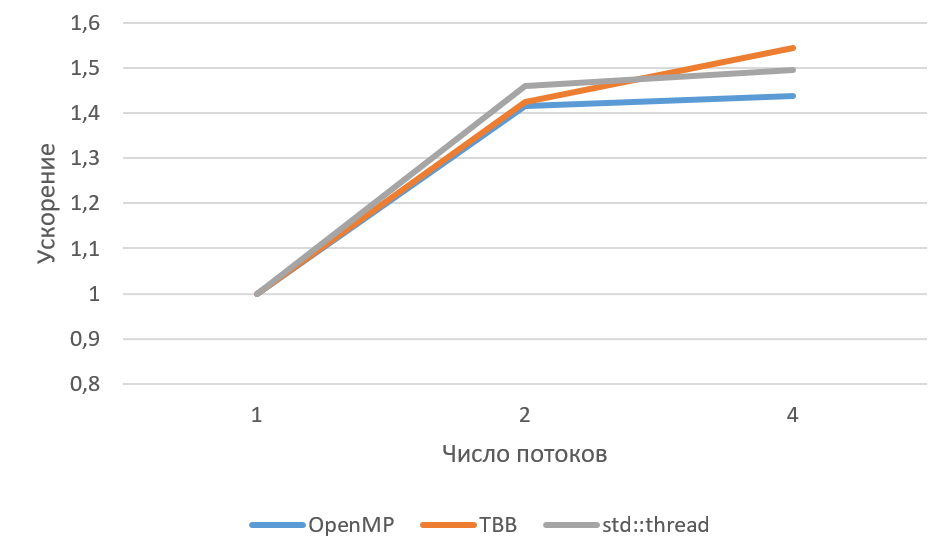
\includegraphics[width=0.99\textwidth]{../../../../modules/reports/konnov_s_radix_sort_odd_even_merge_double/pic.png}
        \caption{Ускорение работы в зависимости от числа потоков на различных версиях программы}
    \end{figure}
    \par Как видно из графика, для всех трёх версий при увеличении количества процессов ускорение работы примерно одинаковое и колеблется около 1.4 при 2 потоках и 1.5 при 4 потоках. Ускорение есть, но его прирост сильно замедляется при увеличении числа потоков. Это связано с большими накладными расходами при использовании чётно-нечётного слияния Бэтчера, которые растут вместе с увеличением числа потоков, так как необходимо сливать большее число частей массива друг с другом.
    \clearpage
    % =============================================
    % Заключение
    % =============================================
    \section*{Заключение}
    \addcontentsline{toc}{section}{Заключение}
    В ходе выполнения лабораторных работ были реализованы последовательная версия алгоритма поразрядной сортировки, рассмотрен алгоритм чётно-нечётного слияния Бэтчера, реализованы параллельные версии сортировки с использованием \verb|OpenMP|, \verb|TBB| и \verb|std::thread|. Была проведена проверка эффективности работы каждой из параллельных версий. В результате проверки был сделан вывод о том, что ускорение есть, но при увеличении числа потоков темпы роста ускорения замедляются из-за наличия больших накладных расходов.

    \newpage
    % =============================================
    % Список литературы
    % =============================================
    \section*{Список литературы}
    \addcontentsline{toc}{section}{Список литературы}
    \begin{enumerate}
        \item Сысоев А.В., Мееров И.Б., Сиднев А.А. Средства разработки параллельных программ для систем с общей памятью. Библиотека Intel Threading Building Blocks. Учебно-методические материалы по программе повышения квалификации «Технологии высокопроизводительных вычислений для обеспечения учебного процесса и научных исследований». Нижний Новгород, 2007, 86 с.
        \item Intel Threading Building Blocks User Guide. URL: \url{https://www.threadingbuildingblocks.org/docs/help/tbb_userguide/parallel_for.html}
        \item Guide into OpenMP: Easy multithreading programming for C++. URL: \url{https://bisqwit.iki.fi/story/howto/openmp/}
    \end{enumerate}

    \newpage
    \section*{Приложение}
    \addcontentsline{toc}{section}{Приложение}

    \subsection*{Исходный код}
    \addcontentsline{toc}{subsection}{Исходный код}

    \subsubsection*{Лабораторная работа №1. Последовательная версия}
    \addcontentsline{toc}{subsubsection}{Лабораторная работа №1. Последовательная версия}
    \lstinputlisting[language=C++, caption=Последовательная версия. Заголовочный файл]{../../../../modules/task_1/konnov_s_radix_sort_odd_even_merge_double/radix_sort_odd_even_merge_double.h}
    \lstinputlisting[language=C++, caption=Последовательная версия. Файл с реализацией]{../../../../modules/task_1/konnov_s_radix_sort_odd_even_merge_double/radix_sort_odd_even_merge_double.cpp}
    \lstinputlisting[language=C++, caption=Последовательная версия. Файл с тестами]{../../../../modules/task_1/konnov_s_radix_sort_odd_even_merge_double/main.cpp}

    \newpage
    \subsubsection*{Лабораторная работа №2. Параллельная версия с использованием OpenMP}
    \addcontentsline{toc}{subsubsection}{Лабораторная работа №2. Параллельная версия с использованием OpenMP}
    \lstinputlisting[language=C++, caption=Параллельная версия с использованием OpenMP. Заголовочный файл]{../../../../modules/task_2/konnov_s_radix_sort_odd_even_merge_double/radix_sort_odd_even_merge_double.h}
    \lstinputlisting[language=C++, caption=Параллельная версия с использованием OpenMP. Файл с реализацией]{../../../../modules/task_2/konnov_s_radix_sort_odd_even_merge_double/radix_sort_odd_even_merge_double.cpp}
    \lstinputlisting[language=C++, caption=Параллельная версия с использованием OpenMP. Файл с тестами]{../../../../modules/task_2/konnov_s_radix_sort_odd_even_merge_double/main.cpp}

    \newpage
    \subsubsection*{Лабораторная работа №3. Параллельная версия с использованием TBB}
    \addcontentsline{toc}{subsubsection}{Лабораторная работа №3. Параллельная версия с использованием TBB}
    \lstinputlisting[language=C++, caption=Параллельная версия с использованием TBB. Заголовочный файл]{../../../../modules/task_3/konnov_s_radix_sort_odd_even_merge_double/radix_sort_odd_even_merge_double.h}
    \lstinputlisting[language=C++, caption=Параллельная версия с использованием TBB. Файл с реализацией]{../../../../modules/task_3/konnov_s_radix_sort_odd_even_merge_double/radix_sort_odd_even_merge_double.cpp}
    \lstinputlisting[language=C++, caption=Параллельная версия с использованием TBB. Файл с тестами]{../../../../modules/task_3/konnov_s_radix_sort_odd_even_merge_double/main.cpp}

    \newpage
    \subsubsection*{Лабораторная работа №4. Параллельная версия с использованием std::thread}
    \addcontentsline{toc}{subsubsection}{Лабораторная работа №4. Параллельная версия с использованием std::thread}
    \lstinputlisting[language=C++, caption=Параллельная версия с использованием std::thread. Заголовочный файл]{../../../../modules/task_4/konnov_s_radix_sort_odd_even_merge_double/radix_sort_odd_even_merge_double.h}
    \lstinputlisting[language=C++, caption=Параллельная версия с использованием std::thread. Файл с реализацией]{../../../../modules/task_4/konnov_s_radix_sort_odd_even_merge_double/radix_sort_odd_even_merge_double.cpp}
    \lstinputlisting[language=C++, caption=Параллельная версия с использованием std::thread. Файл с тестами]{../../../../modules/task_4/konnov_s_radix_sort_odd_even_merge_double/main.cpp}
\end{document}